\section{Methodology}

In this project, we implemented a convolutional denoising autoencoder for removing noise from images. The model consists of two main components: an encoder and a decoder.

The \textbf{encoder} part includes two convolutional layers with 64 filters each, using ReLU activation and 3x3 kernels, followed by max-pooling operations and dropout for regularization. This part compresses the input into a lower-dimensional latent space.

The \textbf{decoder} part mirrors the encoder and consists of convolutional layers followed by upsampling operations. The final output layer uses a sigmoid activation function to produce pixel values in the range [0, 1], matching the normalized input.

The model is trained using binary cross-entropy loss and the Adam optimizer with a batch size of 128 over 15 epochs. The goal is to minimize the reconstruction error between the original and denoised images.

Figure~\ref{fig:flowchart} shows the overall architecture and data flow of the proposed model.

\begin{figure}[ht]
    \centering
    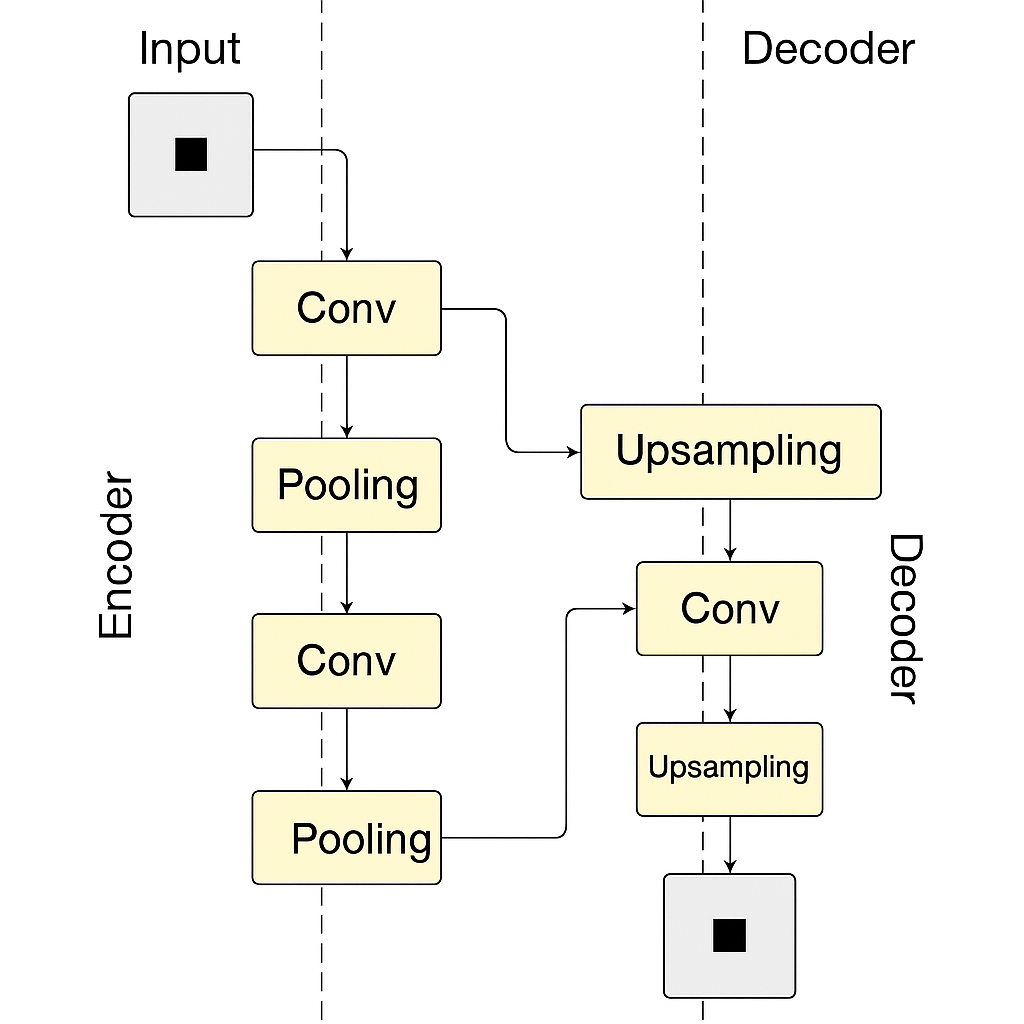
\includegraphics[width=\linewidth]{figures/flowchart.png}
    \caption{Workflow of the convolutional denoising autoencoder.}
    \label{fig:flowchart}
\end{figure}